\documentclass{beamer}
%\documentclass[xcolor=dvipsnames]{beamer}
\usepackage[spanish]{babel}
\usepackage[utf8]{inputenc}
\usepackage{graphicx}
\usepackage{csquotes}

\newcommand{\beamer}{\textsc{beamer}}
\newtheorem{definicion}{Definición}
\newtheorem{ejemplo}{Ejemplo}

%%%%%%%%%%%%%%%%%%%%%%%%%%%%%%%%%%%%%%%%%%%%%%%%%%%%%%%%%%%%%%%%%%%%%%%%%%%%%%%
\title[genetics.js]{
    genetics.js \\
    Framework web de computación evolutiva
}
\author[Cristian Abrante]{Cristian Manuel Abrante Dorta}
\institute[ULL]{Universidad de La Laguna}
\date[21-06-2019]{\today}
%%%%%%%%%%%%%%%%%%%%%%%%%%%%%%%%%%%%%%%%%%%%%%%%%%%%%%%%%%%%%%%%%%%%%%%%%%%%%%%

\usetheme{Madrid}
%\usetheme{Warsaw}

%%%%%%%%%%%%%%%%%%%%%%%%%%%%%%%%%%%%%%%%%%%%%%%%%%%%%%%%%%%%%%%%%%%%%%%%%%%%%%%
\definecolor{pantone254}{RGB}{87,6,140}
\definecolor{pantone3015}{RGB}{0,88,147}
\definecolor{pantone432}{RGB}{56,61,66}
\setbeamercolor*{palette primary}{use=structure,fg=white,bg=pantone254}
\setbeamercolor*{palette secondary}{use=structure,fg=white,bg=pantone3015}
\setbeamercolor*{palette tertiary}{use=structure,fg=white,bg=pantone432}
\setbeamercolor*{palette sidebar primary}{use=structure,fg=pantone254}
\setbeamercolor*{palette sidebar tertiary}{use=structure,fg=pantone3015}
\setbeamercolor*{block title}{bg=pantone3015,fg=white}
\setbeamercolor*{alerted text}{fg=pantone432}
\setbeamercolor*{item projected}{fg=pantone254}
\setbeamercolor*{section in toc shaded}{use=structure,fg=structure.fg}
\setbeamercolor*{section in toc}{fg=pantone3015}
\setbeamercolor*{subsection in toc shaded}{fg=pantone3015}
\setbeamercolor*{subsection in toc}{fg=pantone432}

%%%%%%%%%%%%%%%%%%%%%%%%%%%%%%%%%%%%%%%%%%%%%%%%%%%%%%%%%%%%%%%%%%%%%%%%%%%%%%%
\begin{document}
  
%++++++++++++++++++++++++++++++++++++++++++++++++++++++++++++++++++++++++++++++  
\begin{frame}

  
\includegraphics[width=0.45\textwidth]{pres/img/etsit-logo.png}
  \hspace*{2cm}
  
\includegraphics[width=0.35\textwidth]{pres/img/geneticsjs-logo.png}
  \titlepage

  \begin{scriptsize}
    \begin{center}
     Escuela Superior de Ingeniería y Tecnología \\
     Universidad de La Laguna
    \end{center}
  \end{scriptsize}

\end{frame}
%++++++++++++++++++++++++++++++++++++++++++++++++++++++++++++++++++++++++++++++  

%++++++++++++++++++++++++++++++++++++++++++++++++++++++++++++++++++++++++++++++  
\begin{frame}
  \frametitle{Índice}  
  \tableofcontents[pausesections]
\end{frame}
%++++++++++++++++++++++++++++++++++++++++++++++++++++++++++++++++++++++++++++++  


\section{Motivación y Objetivos}


%++++++++++++++++++++++++++++++++++++++++++++++++++++++++++++++++++++++++++++++  
\begin{frame}

\frametitle{Introducción}
\begin{exampleblock}{}
  {\large ``La gran ventaja de la evolución es la gran cantidad de especies diferentes que ha creado, cada una adaptada a su medio''}
  \vskip5mm
  \hspace*\fill{\small--- A.E. Eiben y J.E. Smith}
\end{exampleblock}
\end{frame}
%++++++++++++++++++++++++++++++++++++++++++++++++++++++++++++++++++++++++++++++  

%++++++++++++++++++++++++++++++++++++++++++++++++++++++++++++++++++++++++++++++  
\begin{frame}

\frametitle{Introducción}

En primer lugar, veremos una clasificación de los problemas en función de su complejidad.

\begin{figure}
    \centering
    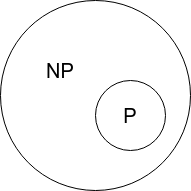
\includegraphics[scale=0.5]{pres/img/introduccion/p-np.png}
    \caption{Representación de las clases de problemas $\mathcal{P}$ y $\mathcal{NP}$}
    \label{fig:p-np}
\end{figure}

\begin{itemize}
    \item \textbf{Clase $\mathcal{P}$}: Se puede encontrar una solución en \textbf{tiempo polinomial}.
    \item \textbf{Clase $\mathcal{NP}$}: Se puede verificar una solución en \textbf{tiempo polinomial}.
\end{itemize}

\end{frame}
%++++++++++++++++++++++++++++++++++++++++++++++++++++++++++++++++++++++++++++++  

%++++++++++++++++++++++++++++++++++++++++++++++++++++++++++++++++++++++++++++++  
\begin{frame}

\frametitle{Introducción}

Dentro de la clase $\mathcal{NP}$, existen una gran cantidad de problemas de \textbf{optimización combinatoria}. \\

\begin{block}{Optimización combnatoria}
 En este tipo de problemas, se trata de optimizar una función objetivo, que depende de una serie de variables \textbf{discretas}, sujetas a un conjunto de restricciones.
\end{block}
\\
Algunos ejemplos de este tipo de problemas:

\begin{itemize}
    \item Problema del viajante de comercio (TSP).
    \item Problema de las ocho reinas.
\end{itemize}
\end{frame}
%++++++++++++++++++++++++++++++++++++++++++++++++++++++++++++++++++++++++++++++  

%++++++++++++++++++++++++++++++++++++++++++++++++++++++++++++++++++++++++++++++  
\begin{frame}

\frametitle{Introducción}

Formalmente, un problema ($P$) de optimización combinatoria se puede definir como una tupla:

\begin{center}
    $P = (S, f, \Omega)$
\end{center}

Donde:

\begin{itemize}
    \item \textbf{Espacio de soluciones} ($S$): Es el conjunto finito y numerable de todas las posibles soluciones al problema.
    \item \textbf{Función objetivo} ($f$): Para cada solución de $S$, devuelve su valor de bondad.
    \begin{center}
        \begin{math}
            f: S \rightarrow \mathbb{R}
        \end{math}
    \end{center}
    \item \textbf{Conjunto de restricciones} ($\Omega$): Conjunto de restricciones que debe satisfacer una solución de s ($s \in S$), para ser válida.
\end{itemize}

\end{frame}
%++++++++++++++++++++++++++++++++++++++++++++++++++++++++++++++++++++++++++++++  

\begin{frame}

\frametitle{Introducción}

El concepto de \textbf{óptimo global} ($s^*$) es la solución para la cual la función objetivo tiene una evaluación más alta:

\begin{center}
    $\forall s \in S, \quad f(s^*) \geq f(s)$ 
\end{center}

Para encontrar esta solución, existen varias opciones:

\begin{itemize}
    \item Enumerar todas las soluciones de $S$. Esto suele ser \textbf{inviable} debido al gran tamaño de este conjunto.
    \item Utilizar una \textbf{exploración inteligente} del espacio de soluciones. Utilizando por ejemplo, \textbf{metaheurísticas}.
\end{itemize}

\end{frame}
%++++++++++++++++++++++++++++++++++++++++++++++++++++++++++++++++++++++++++++++  

\begin{frame}

\frametitle{Introducción}

El concepto de \textbf{óptimo global} ($s^*$) es la solución para la cual la función objetivo tiene una evaluación más alta:

\begin{center}
    $\forall s \in S, \quad f(s^*) \geq f(s)$ 
\end{center}

Para encontrar esta solución, existen varias opciones:

\begin{itemize}
    \item Enumerar todas las soluciones de $S$. Esto suele ser \textbf{inviable} debido al gran tamaño de este conjunto.
    \item Utilizar una \textbf{exploración inteligente} del espacio de soluciones. Utilizando, por ejemplo, \textbf{metaheurísticas}.
\end{itemize}

\end{frame}
%++++++++++++++++++++++++++++++++++++++++++++++++++++++++++++++++++++++++++++++  

\begin{frame}

\frametitle{Introducción}

El concepto de \textbf{óptimo global} ($s^*$) es la solución para la cual la función objetivo tiene una evaluación más alta:

\begin{center}
    $\forall s \in S, \quad f(s^*) \geq f(s)$ 
\end{center}

Para encontrar esta solución, existen varias opciones:

\begin{itemize}
    \item Enumerar todas las soluciones de $S$. Esto suele ser \textbf{inviable} debido al gran tamaño de este conjunto.
    \item Utilizar una \textbf{exploración inteligente} del espacio de soluciones. Utilizando, por ejemplo, \textbf{metaheurísticas}.
\end{itemize}

\end{frame}
%++++++++++++++++++++++++++++++++++++++++++++++++++++++++++++++++++++++++++++++  

\begin{frame}

\frametitle{Introducción}

\begin{block}{Metaheurísticas}
 Las metaheurísticas se centran en encontrar soluciones a problemas de optimización aplicando una búsqueda en el espacio de soluciones ($S$), cuando no se tiene información específica del problema.
\end{block}

Existen muchas técnicas metaheurísticas, que se pueden clasificar según diferentes criterios, sin embargo en este trabajo nos centraremos en la \textbf{computación evolutiva}.

\end{frame}
%++++++++++++++++++++++++++++++++++++++++++++++++++++++++++++++++++++++++++++++  

\begin{frame}

\frametitle{Introducción}

La \textbf{computación evolutiva} es una técnica metaheurística, bio-inpirada y basada en población.\\

Está inspirada en el proceso evolutivo natural, principalmente

\end{frame}
%++++++++++++++++++++++++++++++++++++++++++++++++++++++++++++++++++++++++++++++  

\section{Fundamentos Teóricos}

\begin{frame}
\frametitle{Fundamentos Teóricos}

Se presentarán los antecedentes teóricos y prácticos que apoyan el tema objeto
del trabajo.

\end{frame}
%++++++++++++++++++++++++++++++++++++++++++++++++++++++++++++++++++++++++++++++  

\section{Procedimiento experimental}

\begin{frame}
\frametitle{Procedimiento experimental}

Ha de contar con secciones para la descripción de los experimentos y del material.
También deber haber una sección para los resultados obtenidos y una última de
análisis de los resultados obtenidos.

\end{frame}
%++++++++++++++++++++++++++++++++++++++++++++++++++++++++++++++++++++++++++++++  

\subsection{Descripción de los experimentos}

%++++++++++++++++++++++++++++++++++++++++++++++++++++++++++++++++++++++++++++++  
\begin{frame}
\frametitle{Generación de datos aleatoria}

\begin{ejemplo}
  \begin{itemize}
    \item <1-> Con semilla 1 
    \item <2-> Con semilla 10 
    \item <3> Sin semilla 
  \end{itemize}
\end{ejemplo}

\end{frame}
%++++++++++++++++++++++++++++++++++++++++++++++++++++++++++++++++++++++++++++++  

\subsection{Descripción del material}
%++++++++++++++++++++++++++++++++++++++++++++++++++++++++++++++++++++++++++++++  
\begin{frame}
\frametitle{Hardware y Software}

\begin{ejemplo}
  \begin{enumerate}
    \item
      Descripción del hardware 
      \pause

    \item
      Descripción del software 
  \end{enumerate}
\end{ejemplo}

\end{frame}
%++++++++++++++++++++++++++++++++++++++++++++++++++++++++++++++++++++++++++++++  

\subsection{Resultados obtenidos}
%++++++++++++++++++++++++++++++++++++++++++++++++++++++++++++++++++++++++++++++  
\begin{frame}
\frametitle{Medidas de tiempo y Velocidad}

%------------------------------------------------------------------------------
%--------------------------------------------------------------------------
\begin{table}[!ht]
\begin{center}
\begin{tabular}{|p{25mm}|p{80mm}|} \hline 
\textbf{Tipos } & \textbf{Descripcion} \\ \hline
AAAA &
BBBB
\\
\hline

CCCC &
DDDD
\\
\hline

EEEE &
FFFF
\\
\hline

GGGG &
HHHH
\\
\hline

\end{tabular}
\end{center}
\caption{Tabla resumen de los Tipos}
\label{table:resOthers}
\end{table}


%------------------------------------------------------------------------------

\end{frame}
%++++++++++++++++++++++++++++++++++++++++++++++++++++++++++++++++++++++++++++++  


\subsection{Análisis de los resultados}
%++++++++++++++++++++++++++++++++++++++++++++++++++++++++++++++++++++++++++++++  
\begin{frame}
\frametitle{Diagrama del tiempo y la velocidad}

%------------------------------------------------------------------------------
\begin{figure}[!th]
\begin{center}
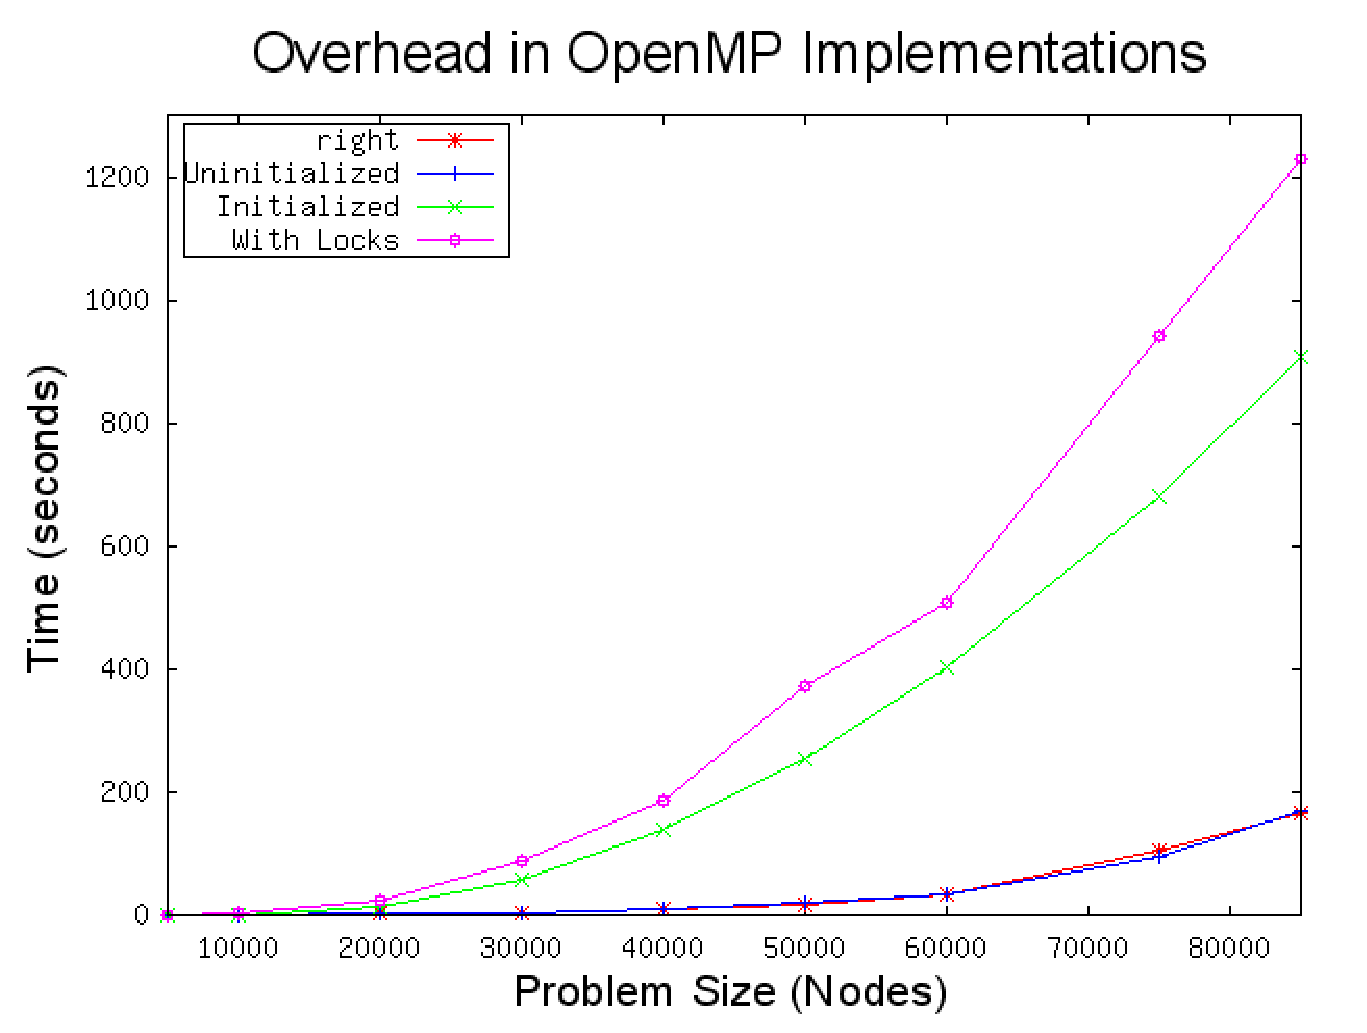
\includegraphics[width=0.75\textwidth]{img/figura1.eps}
\caption{Ejemplo de figura}
\label{fig:1}
\end{center}
\end{figure}
%------------------------------------------------------------------------------

\end{frame}
%++++++++++++++++++++++++++++++++++++++++++++++++++++++++++++++++++++++++++++++  


\section{Conclusiones}

%++++++++++++++++++++++++++++++++++++++++++++++++++++++++++++++++++++++++++++++  
\begin{frame}
\frametitle{Conclusiones}

\begin{ejemplo}
  \begin{enumerate}
    \item
      Conclusión 1
      \pause
    \item
      Conclusión 2
  \end{enumerate}
\end{ejemplo}

\end{frame}
%++++++++++++++++++++++++++++++++++++++++++++++++++++++++++++++++++++++++++++++  

%++++++++++++++++++++++++++++++++++++++++++++++++++++++++++++++++++++++++++++++  
\begin{frame}
  \frametitle{Bibliografía}

  \begin{thebibliography}{10}

    \beamertemplatebookbibitems
    \bibitem[URL: CTAN]{latex} 
    CTAN. {\small $http://www.ctan.org/$}

    \beamertemplatebookbibitems
    \bibitem[Tantau, 2005]{beamer} 
    Tantau, Till. 
    \emph{User's Guide to the \beamer{} Class, Version 3.06, 2005} 
    {\small $http://ctang.tug.org/tex-archive/macros/latex/contrib/beamer$}


  \end{thebibliography}
\end{frame}


%++++++++++++++++++++++++++++++++++++++++++++++++++++++++++++++++++++++++++++++  

\end{document}
